%%
%% Copyright 2022 OXFORD UNIVERSITY PRESS
%%
%% This file is part of the 'oup-authoring-template Bundle'.
%% ---------------------------------------------
%%
%% It may be distributed under the conditions of the LaTeX Project Public
%% License, either version 1.2 of this license or (at your option) any
%% later version.  The latest version of this license is in
%%    http://www.latex-project.org/lppl.txt
%% and version 1.2 or later is part of all distributions of LaTeX
%% version 1999/12/01 or later.
%%
%% The list of all files belonging to the 'oup-authoring-template Bundle' is
%% given in the file `manifest.txt'.
%%
%% Template article for OXFORD UNIVERSITY PRESS's document class `oup-authoring-template'
%% with bibliographic references
%%

%%%CONTEMPORARY%%%
\documentclass[unnumsec,webpdf,contemporary,large]{oup-authoring-template}%
%\documentclass[unnumsec,webpdf,contemporary,large,namedate]{oup-authoring-template}% uncomment this line for author year citations and comment the above
%\documentclass[unnumsec,webpdf,contemporary,medium]{oup-authoring-template}
%\documentclass[unnumsec,webpdf,contemporary,small]{oup-authoring-template}

%%%MODERN%%%
%\documentclass[unnumsec,webpdf,modern,large]{oup-authoring-template}
%\documentclass[unnumsec,webpdf,modern,large,namedate]{oup-authoring-template}% uncomment this line for author year citations and comment the above
%\documentclass[unnumsec,webpdf,modern,medium]{oup-authoring-template}
%\documentclass[unnumsec,webpdf,modern,small]{oup-authoring-template}

%%%TRADITIONAL%%%
%\documentclass[unnumsec,webpdf,traditional,large]{oup-authoring-template}
%\documentclass[unnumsec,webpdf,traditional,large,namedate]{oup-authoring-template}% uncomment this line for author year citations and comment the above
%\documentclass[unnumsec,namedate,webpdf,traditional,medium]{oup-authoring-template}
%\documentclass[namedate,webpdf,traditional,small]{oup-authoring-template}

%\onecolumn % for one column layouts

%\usepackage{showframe}

\graphicspath{{Fig/}}

% line numbers
%\usepackage[mathlines, switch]{lineno}
%\usepackage[right]{lineno}
% Package used  
\usepackage{graphicx}
\usepackage{hyperref}
\usepackage{subcaption}
\usepackage{fancyvrb}
\usepackage{xcolor}
\hypersetup{
    colorlinks,
    linkcolor={red!50!black},
    citecolor={blue!50!black},
    urlcolor={blue!80!black}
}

%\usepackage[style=authoryear, maxbibnames=2]{biblatex}
%\addbibresource{reference.bib}
%\AtEveryBibitem{\clearfield{month}}
%\AtEveryBibitem{\clearfield{day}}
%\AtEveryBibitem{\clearfield{doi}}
%\AtEveryBibitem{\clearfield{issn}}
%\AtEveryBibitem{\clearfield{pages}}

\theoremstyle{thmstyleone}%
\newtheorem{theorem}{Theorem}%  meant for continuous numbers
%%\newtheorem{theorem}{Theorem}[section]% meant for sectionwise numbers
%% optional argument [theorem] produces theorem numbering sequence instead of independent numbers for Proposition
\newtheorem{proposition}[theorem]{Proposition}%
%%\newtheorem{proposition}{Proposition}% to get separate numbers for theorem and proposition etc.
\theoremstyle{thmstyletwo}%
\newtheorem{example}{Example}%
\newtheorem{remark}{Remark}%
\theoremstyle{thmstylethree}%
\newtheorem{definition}{Definition}

\begin{document}

\journaltitle{Journal Title Here}
\DOI{DOI HERE}
\copyrightyear{2022}
\pubyear{2019}
\access{Advance Access Publication Date: Day Month Year}
\appnotes{Paper}

\firstpage{1}

%\subtitle{Subject Section}

\title[LRNBuilder]{LRNBuilder: A System for the Modular Construction of Linear Reaction Networks and their Transfer Functions}

\author[1,$\ast$]{First Author}


\authormark{Author Name et al.}

\address[1]{\orgdiv{Department}, \orgname{Organization}, \orgaddress{\street{Street}, \postcode{Postcode}, \state{State}, \country{Country}}}


\corresp[$\ast$]{Corresponding author. \href{email:email-id.com}{email-id.com}}

\received{Date}{0}{Year}
\revised{Date}{0}{Year}
\accepted{Date}{0}{Year}

%\editor{Associate Editor: Name}

%\abstract{
%\textbf{Motivation:} .\\
%\textbf{Results:} .\\
%\textbf{Availability:} .\\
%\textbf{Contact:} \href{name@email.com}{name@email.com}\\
%\textbf{Supplementary information:} Supplementary data are available at \textit{Journal Name}
%online.}

\abstract{Most reaction networks are nonlinear in the sense that their dynamics are described by a system of nonlinear differential equations. In contrast, linear reaction networks (LRN) have dynamics that are described by a system of linear of differential equations. LRNs have appeal because they have an exact solution in the time domain, and so are amenable to use in systems for designing and/or modification to achieve desired goals related to stability, oscillations, settling times, and regulation. Herein, we on single-input, single-output (SISO) linear reaction networks (SLRN).
Key results are:
\begin{enumerate}
    \item Nonlinear reaction networks can be approximated with arbitrary accuracy by a linear reaction network.
    \item The transfer functions are derived for SLRNs that are constructed using the following operations on other SLRNs: concatenation, branch-join, scaling, and (feedback) loops.
    \item We implement LRNBuilder, a system that builds SLRNs constructed using these operations.
    \item We develop an algorithm for constructing an SLRN from a transfer function that is a rational polynomial.
    \item We define modules that are sufficient to construct transfer functions for composed modules and generate reaction networks.
\end{enumerate}}
\keywords{keyword1, Keyword2, Keyword3, Keyword4}

% \boxedtext{
% \begin{itemize}
% \item Key boxed text here.
% \item Key boxed text here.
% \item Key boxed text here.
% \end{itemize}}

\maketitle


\section{Introduction}
Here is a citation (\cite{al2002handgrip}).
\begin{enumerate}

%%%%%%%%%%%
\item
Motivation
\begin{enumerate}
\item Create approximations to nonlinear reaction networks
that are easily analyzed for properties such as stability, oscillations,
settling times, DC gain. Doing so provides the following benefits:
\item Ways that an existing network can be transformed.
\item Identification of functions of biological systems by analyzing
composition of biochemical networks
\item 
Applications to synthetic biology
\end{enumerate}

%%%%%%%%%%%
\item Prior work

%%%%%%%%%%%
\item Challenges
\begin{enumerate}
\item
retroactivity
\end{enumerate}

%%%%%%%%%%%
\item Contributions
\end{enumerate}



\section{Methods}\label{methods}
\begin{enumerate}
\item
Motivation: 
Arbitrary real-valued functions can be approximated by a fourier transform,
and the fourier transform is a subset of the Laplace Transform (where the real part is 0).
\item
This analysis is limited to SISO and transfer functions that
are rational polynomials of $s$ with real coefficients.
\item
Evaluations: (a) can approximate complex simulations; (b) composed models have predictable transfer functions.
\item
Create a {\em sufficient} set of operations such that can
approximate complex simulations.
\end{enumerate}



\section{Results}\label{results}
\subsection{SISO Linear Reaction Networks}

We use subscripted and superscripted $S$ to indicate chemical species. Where there is no confusion, we use the same symbol for its concentration as well. In contexts where there may be confusion between the name and its concentration, we explicitly indicate a concentration using square brackets. For example, $[S_0]$ is the concentration of species $S_0$.

A {\bf reaction} is a four tupleexpressed as $S_I \xrightarrow{k} m S_O$
indicates the transformation of mass from species $S_I$ to $m$ molecules of $S_O$
using mass action with the kinetic constant $k$. If $k < 0$,
then $S_O$ is transformed into $S_I$; that is, $S_O \xrightarrow{-k} S_I$.
If $S_I = \emptyset$ or $S_O = \emptyset$, then this a boundary reaction.
For an input boundary, $k_I$ is a fixed rate.
If $S_O = \emptyset$, then this is a degradation reaction.

Let $\mathcal{R}$ be a set of reactions, and let
$\mathcal{S}$ be the set of all reactants and products in $\mathcal{R}$.
$S_I$ is the input species for the network.
We require that $S_I$ never appear as a product in the reaction network.
$S_O$ is the output species.
We require that $S_O$ never appears as a reactant in the reaction network.
A {\bf SISO Linear Reaction Network (SLRN)} is
a 5-tuple
$<\mathcal{R}, S_I, S_O, k_I, k_O>$ where:
\begin{itemize}
    \item $\mathcal{R}$ is a set of reactions.
    \item 
    $S_I, S_O \in \mathcal{S}$ are input and output species.
    \item $k_I S_I$ is the rate at which the input is consumed
    by the SLRN.
    \item $k_O S_O$ is the rate at which the output is degraded by the SLRN.
\end{itemize}
Sometimes, we work with multiple SLRNs. Components of networks are indicated by a
capital letter superscript.
For example, for network $A$, we have the 5-tuple
$<\mathcal{R}^A, S^A_I, S^A_O, k^A_I, k^A_O>$.

\subsubsection{Sequential Reaction Network}

We start with a sequential network with $N$ stages.
There are $N$ stages with an input and output. The input is $S_0$ and the output is $S_N$. Formally, we have
\begin{eqnarray}
s S_n (s) & =&  k_{n-1} S_{n-1} (s) - (k_n + k^{\prime}) S_n (s) ,~ n>0
\end{eqnarray}

From this, we derive the transfer function for the network.
\begin{align}
S_n (s) & = & \frac{k_{n-1} S_{n-1}}{s + k_n + k^{\prime}_n} \nonumber \\
S_1 (s) & = & \frac{k_0 S_0}{s + k_1 + k^{\prime}_1} \nonumber \\
S_2 (s) & = & \frac{k_1 S_1}{s + k_2 + k^{\prime}_2} \nonumber \\
  & = & \frac{k_1 k_0 S_0}{(s + k_2 + k^{\prime}_2)(s + k_1 + k^{\prime}_1)}
\end{align}

\begin{eqnarray}
S_N (s) & = & \frac{S_0 (s) \prod_{n=0}^{N-1} k_n }{\prod_{n=1}^N(s + k_n + k^{\prime}_n)} \nonumber \\
    & = &  \frac{ k_0 }{s  +  k^{\prime}_N}  
    \frac{\prod_{n=1}^{N-1} k_n }{\prod_{n=1}^{N-1}(s + k_n + k^{\prime}_n)} S_0(s) \nonumber \\
G (s) & = &  \frac{ k_0 }{s  +  k^{\prime}_N}  
    \frac{\prod_{n=1}^{N-1} k_n }{\prod_{n=1}^{N-1}(s + k_n + k^{\prime}_n)}
\end{eqnarray}
where $k_N = 0= k^{\prime}_0$.

\begin{figure}
        \centering
         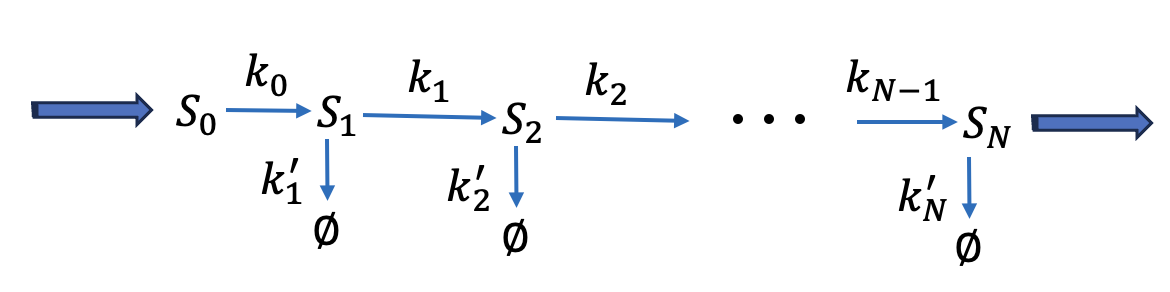
\includegraphics[scale=0.4]{figures/sequential_network.png}
          \caption[]{An $N$ stage sequential network.}
         \label{fig:sequential_network}
\end{figure}


%%%%%%%%%%%%%%%%%
\subsection{Operations on SISO Reaction Networks}
These are operations applied to SLRNs and produce a new SLRN.
In the sequel, $A, B$ are SLRNs.
%%%%%%%%%%%%%%%%%%%%%%%%%%%%%%%%

\subsubsection{concatenate}
\begin{figure}
         \centering
         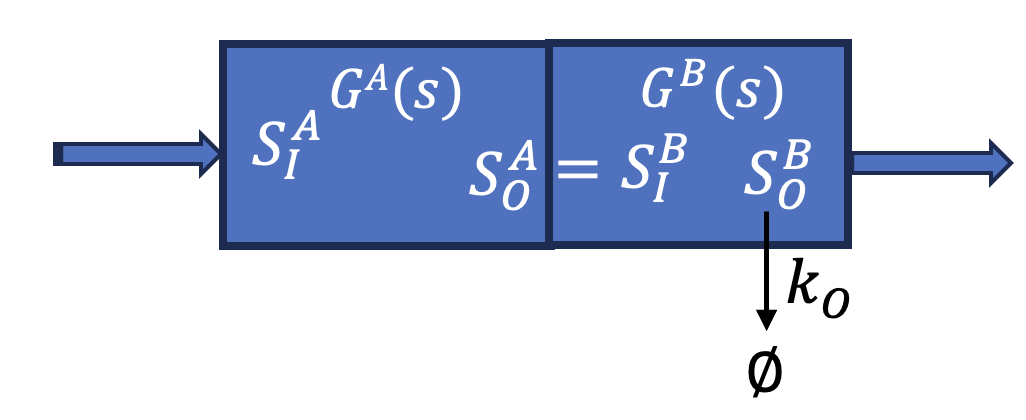
\includegraphics[scale=0.3]{figures/concatenate.png}
          \caption[]{Concatenate operation on networks $A$ and $B$.}
         \label{fig:concatenate}
\end{figure}

{\bf Concatenate} is an asymmetric, binary operation.
Let $A, B$ be such that $\mathcal{S}^A \bigcap \mathcal{S}^B =
\{ S^A_O \} = \{ S^B_I \}$. 
Concatenate applied these SLRNs, denoted by $A \circ  B$,
and produces
the following SLRN:
\begin{itemize}
\item $S_I =S^A_I$
\item $S_O = S^B_O$
\item $\mathcal{R} = \mathcal{R}^A \bigcup \mathcal{R}^B$
\item $k_I = k^A_I$
\item $k_O = k^B_O$
\end{itemize}

Transfer function of the {\em concatenate} operation.
$$G(s) = G^A(s) G^B(s)\frac{s + k^A_O}{s+ k^B_I + k^A_O}$$.

%%%%%%%%%%%%%%%%%
\subsubsection{Branchjoin}
\begin{figure}
         \centering
         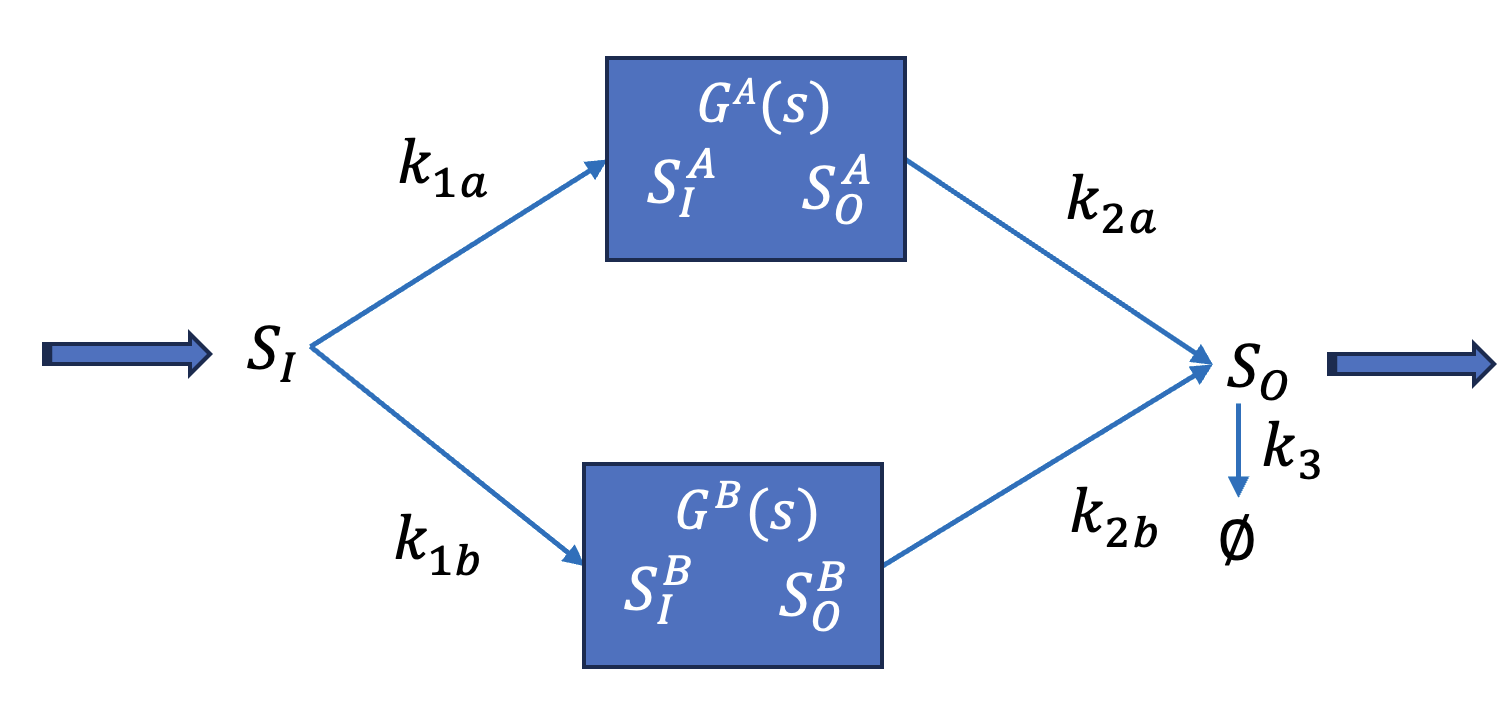
\includegraphics[scale=0.3]{figures/branchjoin.png}
          \caption[]{Branchjoin operation on networks $A$ and $B$.}
         \label{fig:branchjoin}
\end{figure}

{\bf Branchjoin} is a symmetric, binary operation on SLRNs $A, B$ for which
$S^A \bigcap S^B = \emptyset$.
$branchjoin(A, B; k_{1a}, k_{1b}, k_{2a}, k_{2b}, k_3)$
produces:
\begin{itemize}
\item $S_I$, a new species
\item $S_O$, a new species
\item $\mathcal{R} = \mathcal{R}^A \bigcup \mathcal{R}^B$ and the following reactions.
\begin{itemize}
\item
$S_I \xrightarrow{k_{1a}} S^A_I$
\item $S_I \xrightarrow{k_{1b}} S^B_I$
\item
$S^A_O \xrightarrow{k_{2a}} S_O$
\item
$S^B_O \xrightarrow{k_{2b}} S_O$
\item
$S_O \xrightarrow{k_3} \emptyset$
\end{itemize}
\item $k_I = k_{1a} + k_{1b}$
\item $k_O = k_3$
\end{itemize}

Transfer function of the {\em branchjoin} operation.
Let $N_1, N_2$ be reaction networks with transfer functions $G^A(s), G^B(s)$. Let $H(s)$ be the transfer function for $N^A + N^B$.

We begin by writing the state equations based on the flow diagram.
   \begin{eqnarray}
   s S^A_I (s) & = & k_{1a} S_I(s) - k^A_I S^A_I (s) \nonumber \\
   s S^B_I (s) & = & k_{1b} S_I(s) - k^B_I S^B_I (s) \nonumber \\
   S^A_O (s) & = &  S^A_I (s) G^A(s) \frac{s + k^A_O}{s + k^A_O + k_{2a}} \nonumber \\
   S^B_O (s) & = & S^B_I (s)  G^B(s) \frac{s + k^B_O}{s + k^B_O + k_{2b}} \nonumber \\
   sS_O (s) & = & k_{2a} S^A_O(s) + k_{2b} S^B_O(s) - k_3 S_O(s)
   \end{eqnarray}

The following are dervied from the state equations.
\begin{eqnarray}
S^A_I(s) & = & \frac{k_{1a} S_I (s)}{s + k^A_I} \nonumber \\
S^B_I(s) & = & \frac{k_{1b} S_I (s)}{s + k^B_I} \nonumber \\
S^A_O & = & \frac{k_{1a} S_I (s)}{s + k^A_I} G^A(s) \frac{s + k^A_O}{s + k^A_O + k_{2a}} \nonumber\\
   & = & \frac{k_{1a}}{s + k^A_I} \frac{s + k^A_O}{s + k^A_O + k_{2a}}  G^A(s) S_I (s) \nonumber \\
S^B_O
   & = & \frac{k_{1b}}{s + k^B_I} \frac{s + k^B_O}{s + k^B_O + k_{2b}}  G^B(s) S_I (s) \nonumber \\
S_O (s) & = & \frac{k_{2a} S^A_O(s) + k_{2b} S^B_O(s) }{s + k_3} \nonumber \\
G(s) & = & \frac{k_{1a} k_{2a} (s + k^A_O) \beta(s) G^A(s) }{\alpha(s) \beta(s) (s + k_3)} \nonumber \\
& & +  \frac{k_{1b}  k_{2b} (s + k^B_O)\alpha(s) G^B(s) }{\alpha(s) \beta(s) (s + k_3)} \\
\end{eqnarray}

$\alpha(s) = (s + k^A_I) (s + k^A_O + k_{2a})$ and
$\beta(s) = (s + k^B_I) (s + k^B_O + k_{2b})$.

%%%%%%%%%%%%%%%%%
\subsubsection{Scale}
\begin{figure}
         \centering
         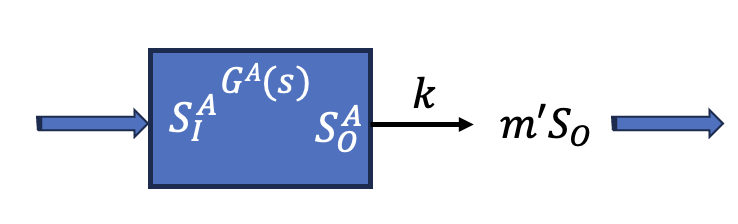
\includegraphics[scale=0.4]{figures/scale.png}
          \caption[]{Scale operation on network $A$.}
         \label{fig:scale}
\end{figure}
{\bf Scale} is a unary operation.
$scale(A, k, m)$ produces 
\begin{itemize}
\item $S_I = S^A_O$
\item $S_O$, a new species
\item $R = \mathcal{R}^A \bigcup \{S_O \xrightarrow{k} \frac{m}{k} S_O\}$
\item $k_I = k$
\item $k_O = 0$
\end{itemize}

Transfer function of the {\em scale} operation.
Scale is a concatenation.
The transfer function for the scale reaction is
$H(s) = \frac{km/k } {s}$, and the concatenation with $A$
has the transfer function
$G(s) = G^A(s) \frac{k^A_O}{k^A_O} H(s)$ and so
$G(0) = m$.


%%%%%%%%%%%%%%%%%
\subsubsection{Loop}

\begin{figure}
         \centering
         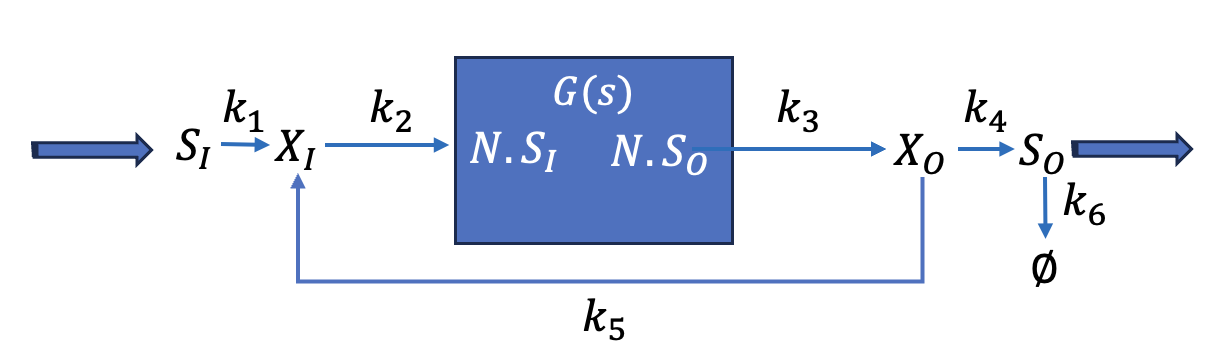
\includegraphics[scale=0.4]{figures/loop.png}
          \caption[]{Loop operation on network $A$.}
         \label{fig:concatenate}
\end{figure}
{\bf Loop} is a unary operation.
$loop(A, S_I, S_O, k_1, k_2, k)$ is a unary operation that produces
the SLRN:
\begin{itemize}
\item $S_I$ is a new species.
\item $S_O$ is a new species.
\item $\mathcal{R} = \mathcal{R}^A \bigcup$ the following
\begin{itemize}
\item $S_I \xrightarrow{k_1} S^A_I$
\item $S^A_O \xrightarrow{k} S_I$
\item $S^A_O \xrightarrow{k_2} S_O$
\end{itemize}
\item $k_I = k^A_I$
\item $k_O = k^A_O + k$
\end{itemize}

The following are the state equations of this system.
\begin{eqnarray}
s S_O (s) & = & k_3 S^A_O (s) - (k_4 + k_5) S_O \nonumber \\
S_O & = & \frac{k_3 S^A_O(s)}{s + k_4 + k_5} \\
s S^A_I(s) & = & k_2 X_I(s) - k^A_I S^A_I(s) \nonumber \\
S^A_I(s) & = & \frac{k_2 X_I(s)}{s + k^A_I} \\
s X_I (s) & = & k_5 S_O(s) + k_1 S_I (s) - k_2 X_I (s) \nonumber \\
X_I(s) & = & \frac{k_5 S_O(s) + k_1 S_I (s)}{s + k_2} \\
S^A_O(s) & = & S^A_I(s) G^A(s) \frac{s + k^A_O}{s + k^A_O + k_3}
\end{eqnarray}
We manipulate the state equations to derive the transfer function of
the loop operation.
This analysis is contained in
Fig.~\ref{fig:loop-derivation}

\begin{figure*}
\begin{eqnarray}
s S_O (s) & = & k_3   G^A(s) \frac{s + k^A_O}{ s + k^A_O + k_3}  S^A_I(s) - (k_4  + k_5) S_O (s) \nonumber \\
& = &
  k_2 k_3  G(s) \frac{s + k^A_O}{(s + k^A_O + k_3)(s + k^A_I)} X_I(s)
   -(k_4 S + k_5 )S_O (s) \nonumber \\
& = &
k_2 k_3  G^{\prime}(s)X_I(s) - (k_4 + k_5) S_O(s)  \nonumber \\
S_O & = &  \frac{k_2 k_3  G^{\prime}(s) X_I(s)}{s + k_4 + k_5  }  \nonumber \\
    & = &  \frac{k_2 k_3  G^{\prime}(s)}{s + k_4 + k_5  } \frac{k_5 S_O(s) + k_1 S_I (s)}{s + k_2} \nonumber \\
(s + k_4 + k_5)(s + k_2)S_O & = &
   k_2 k_3  G^{\prime}(s) (k_5 S_O(s) + k_1 S_I(s))
    \nonumber \\
S_O & = &  \frac{k_1 k_2 k_3  G^{\prime}(s) S_I(s)}{(s + k_4 + k_5)(s + k_2) + k_2 k_3 k_5 G^{\prime}(s)} \nonumber \nonumber \\
H(s) & = & \frac{k_1 k_2 k_3  G^{\prime}(s)}{(s + k_4 + k_5)(s + k_2) + k_2 k_3 k_5 G^{\prime}(s)} \nonumber \\
    & = & \frac{k_1 k_2 k_3  (s + k^A_O) G^A(s)}{(s + k^A_O + k_3)(s + k^A_I)(s + k_4 + k_5)(s + k_2) + k_2 k_3 k_5 (s + k^A_O)G(s)}
\end{eqnarray}
\caption{Loop derivations}\label{fig:loop-derivation}
\end{figure*}

%%%%%%%%%%%%%%%%%%%%%%%%%%%%%
\section{Discussion}\label{discussion}
\begin{enumerate}

%%%%%%%%%%%%%
\item
Principles
\begin{enumerate}
\item 
Adding poles and zeros
\item
Modular design of network so can account for retroactivity
\item
Technique for adjusting transfer functions for retroactivity
\end{enumerate}

\end{enumerate}

\section{Conclusions}

\section{Issues}
\begin{enumerate}
    \item Should I consider MIMO components? This seems possible, but it means more complex state models?
    \begin{enumerate}
    \item There should be separate $branch$ and $join$ operations.
    \item Inputs and outputs should be indexed, $S_{I_i}$, $S_{O_j}$.
    \end{enumerate}
    \item First develop the SISO theory?
\end{enumerate}

\bibliographystyle{plainnat}
\bibliography{reference}
\end{document}
